\newcommand{\headernode}[1]{\pixelnode{gray!50!white}{#1}}
\newcommand{\pixelnode}[2]{\node[fill=#1]{#2};}

\newcommand{\cpyellow}{yellow}
\newcommand{\cpred}{red}
\newcommand{\cpbrown}{brown}
\newcommand{\cpgreen}{green}
\newcommand{\cpblue}{blue}

\newcommand{\cyellow}{\pixelnode{\cpyellow}{0}}
\newcommand{\cred}{\pixelnode{\cpred}{1}}
\newcommand{\cbrown}{\pixelnode{\cpbrown}{2}}
\newcommand{\cgreen}{\pixelnode{\cpgreen}{3}}
\newcommand{\cblue}{\pixelnode{\cpblue}{4}}

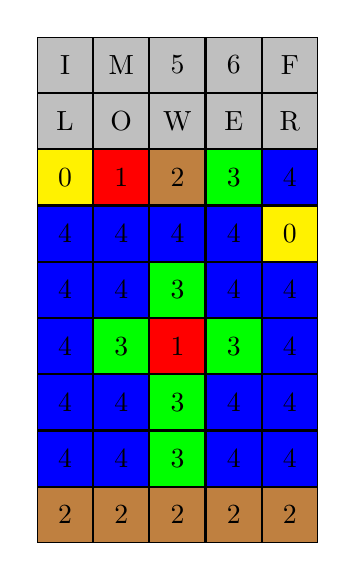
\begin{tikzpicture}

  \matrix[nodes={rectangle,draw,minimum size=7mm}]
  {
    \headernode{I} &  \headernode{M} & \headernode{5} & \headernode{6} & \headernode{F} \\
    \headernode{L} & \headernode{O} & \headernode{W} & \headernode{E} & \headernode{R} \\
    \cyellow & \cred & \cbrown & \cgreen & \cblue \\
    \cblue & \cblue & \cblue & \cblue & \cyellow \\
    \cblue & \cblue & \cgreen & \cblue & \cblue \\
    \cblue & \cgreen & \cred & \cgreen & \cblue \\
    \cblue & \cblue & \cgreen & \cblue & \cblue \\
    \cblue & \cblue & \cgreen & \cblue & \cblue \\
    \cbrown & \cbrown & \cbrown & \cbrown & \cbrown \\
  };

\end{tikzpicture}
